\documentclass{article}
\usepackage{mathtools}
\usepackage[top=2in, bottom=1.5in, left=1in, right=1in]{geometry}
\usepackage{graphicx}
\usepackage[normalem]{ulem}
\usepackage{fancyhdr}
\usepackage{enumerate}
\pagestyle{fancyplain}

\lhead{PHYS 152 Section 10}

\rhead{A. Shawn Bandy 
(003635396)}

\begin{document}
\title{Lab \#4A:  Capacitance: An Introduction}
\author{A. Shawn Bandy}
\date{March 4\textsuperscript{th}, 2013}
\maketitle
\begin{abstract}
A capacitor is an electrical component made of two or more conductive plates separated by dielectric material.  When a voltage potential is applied to the conductors, a static electric field is generated across the dielectric material.  Capacitance is the ratio of the electric charge on each conductor plate to the potential difference between them.\footnote{"Capacitor." {\it{Wikipedia, The Free Encyclopedia.}} Wikimedia Foundation, Inc. 5 March 2013. Web. 5 March 2013.}  \\

In this lab, we estimate the capitance of an unknown capactior by measuring the voltage at 10 second intervals as it discharged through two known resistors.  
\end{abstract}
\section{Data and Data Tables}

\begin{description}

\item[DATA SHEET \#1] \hfill \\
Measurements involving two nominal 10k($\Omega$) resistors.\
\begin{description}
\item[1. Measurement by meter of R1] = 10.17 k$\Omega$  \
\item[2. Measurement by meter of R2] = 10.33 k$\Omega$  \
\item[3. Measurement by meter of R1 + R2] = 20.4 k$\Omega$  \\
\end{description}
\begin{samepage}
\textbf{Table 1.1 Discharge Through 20k$\Omega$ Resistor } \
{\small{
\begin{center}
	\begin{tabular}{| l | l | l | l | l | l | }
	\hline
Time (sec) & Voltage &  $\Delta$-Voltage & ln($\Delta$-Voltage) \\ \hline
0	&	9.95	&	0	&	0	\\	\hline
10	&	9.13	&	0.82	&	-0.1984509387	\\	\hline
20	&	8.53	&	0.6	&	-0.5108256238	\\	\hline
30	&	7.94	&	0.59	&	-0.5276327421	\\	\hline
40	&	7.4	&	0.54	&	-0.6161861394	\\	\hline
50	&	6.92	&	0.48	&	-0.7339691751	\\	\hline
60	&	6.45	&	0.47	&	-0.7550225843	\\	\hline
70	&	6.03	&	0.42	&	-0.8675005677	\\	\hline
80	&	5.63	&	0.4	&	-0.9162907319	\\	\hline
90	&	5.25	&	0.38	&	-0.9675840263	\\	\hline
100	&	4.91	&	0.34	&	-1.0788096614	\\	\hline
110	&	4.58	&	0.33	&	-1.1086626245	\\	\hline
120	&	4.2	&	0.38	&	-0.9675840263	\\	\hline
130	&	3.99	&	0.21	&	-1.5606477483	\\	\hline
140	&	3.74	&	0.25	&	-1.3862943611	\\	\hline



	\end{tabular}
\end{center}
}}
\end{samepage}
\textbf{Table 1.2 Discharge Through 20k$\Omega$ Resistor } \
{\small{
\begin{center}
	\begin{tabular}{| l | l | l | l |}
	\hline
FROM&SLOPE $\frac{k\Omega}{\mu F}$& TIME CONSTANT, RC (sec)&CAPACITANCE C $\mu$F \\ \hline
Slope of line fitted to ln($\Delta$-Voltage)  &-0.007063676&141.568&6.93961\\ \hline
Slope between 30s and 120s&-0.00689192&143.078&7.01363\\ \hline
	\end{tabular}
\end{center}
\% difference: 1.0663 \\
}}

\item[DATA SHEET \#2] \hfill \\
Measurement by meter of resistor used in this circuit = 10.32 k$\Omega$ \\
\textbf{Table 2.2 Discharge Through 10k$\Omega$ Resistor } \
{\small{
\begin{center}
	\begin{tabular}{| l | l | l | l | l | l | }
	\hline
Time (sec) & Voltage &  $\Delta$-Voltage & ln($\Delta$-Voltage) \\ \hline
0	&	9.95	&	0	&	0	\\	\hline
10	&	8.38	&	1.57	&	0.4510756194	\\	\hline
20	&	7.22	&	1.16	&	0.1484200051	\\	\hline
30	&	6.29	&	0.93	&	-0.0725706928	\\	\hline
40	&	5.45	&	0.84	&	-0.1743533871	\\	\hline
50	&	4.74	&	0.71	&	-0.3424903089	\\	\hline
60	&	4.14	&	0.6	&	-0.5108256238	\\	\hline
70	&	3.6	&	0.54	&	-0.6161861394	\\	\hline
80	&	3.15	&	0.45	&	-0.7985076962	\\	\hline
90	&	2.75	&	0.4	&	-0.9162907319	\\	\hline
100	&	2.39	&	0.36	&	-1.0216512475	\\	\hline
110	&	2.1	&	0.29	&	-1.237874356	\\	\hline
120	&	1.83	&	0.27	&	-1.30933332	\\	\hline
130	&	1.61	&	0.22	&	-1.5141277326	\\	\hline
140	&	1.4	&	0.21	&	-1.5606477483	\\	\hline

	\end{tabular}
\end{center}
}}
\textbf{Table 2.2 Discharge Through 10k$\Omega$ Resistor } \
{\small{
\begin{center}
	\begin{tabular}{| l | l | l | l |}
	\hline
FROM&SLOPE $\frac{k\Omega}{\mu F}$& TIME CONSTANT, RC (sec)&CAPACITANCE C $\mu$F \\ \hline
Slope of line fitted to ln($\Delta$-Voltage)&-0.001472928&67.892&6.57868\\ \hline
	\end{tabular}
\end{center}
}}
\end{description}
\section{Graphs}\hfill\\
\begin{samepage}
\textbf{Discharge through 20 K$\Omega$ Resistor} \hfill \\
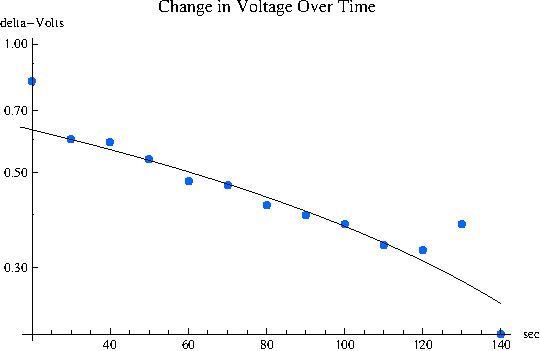
\includegraphics{lab5_graph1}\\ \\
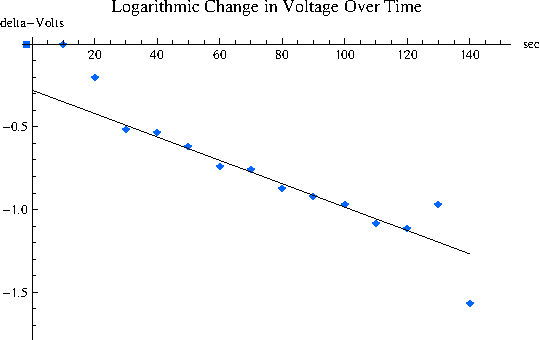
\includegraphics{lab5_graph2}\\
\end{samepage}
\begin{samepage}
\nopagebreak
\textbf{Discharge through 10 K$\Omega$ Resistor} \hfill \\
\nopagebreak
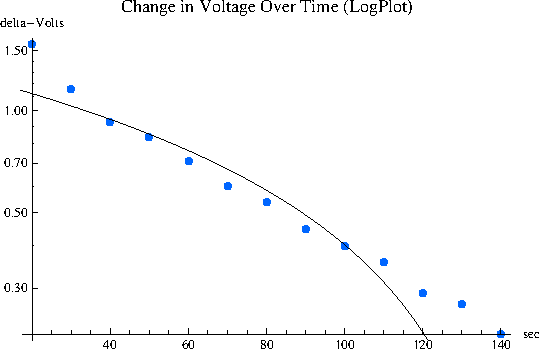
\includegraphics{lab5_graph3}\\ \\
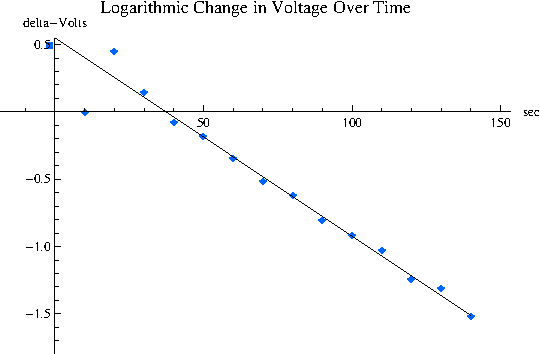
\includegraphics{lab5_graph4}\\
\end{samepage}

\begin{samepage}
\section{Results}\hfill\\
Discharging through 20k$\Omega$ resistors, we estimate the capacitance at 6.93$\mu$F using ordinary least squares to estimate $-\frac{1}{RC}$.  Discharging through a 10k$\Omega$ resistor, we estimate the capacitance to be 6.58$\mu$F.  The percent difference between these two estimates is \%5.32.  
\end{samepage}
\begin{samepage}
\section{Discussion}\hfill\\
\nopagebreak
We applied 9.55 volts from a DC power supply to a capacitor with unknown capacitance.  Voltage was measured with a digital multimeter.  We then disconnected the power supply and quickly replaced with two measured resistors (combined 20.4k$\Omega$) in series.  At the point that the circuit was closed we started timer on a provided stopwatch.  Every ten seconds, for a total of 140 seconds, we measured and recorded the voltage.  We then repeated the procedure with one resistor, measured at 10.33k$\Omega$.  \\ \\
Because the change in voltage of the capacitor over time decays exponentially at rate of $-\frac{t}{RC}$ we can estimate the capacitance C, given that resistance R and time is known. \\
\begin{center}
For and ideal capactior: \\
$\Delta V_c = \Delta V_{batt} * e^{-\frac{t}{RC}}$\\
Taking the natural logarithm of both sides:\\
$ln(\Delta V_c )= ln(\Delta V_{batt} )* -t{\frac{1}{RC}}$ \\ 
Where ${\frac{1}{RC}}$ is the "slope" of the fitted line for $ln(\Delta V_c )$. \\
\end{center}
Using this equation, I estimated the slope using two methods for the resistors in series.  The first was using ordinary least squares and the second was taking two end points.  This yielded slightly different results with a percent difference of \%1.063.  For the single resistor, I used OLS only.  In both cases, I used only measurements from 30 seconds to 120 seconds as both thelab  procedure and the measurements indicated that the first and last measurements clearly do not conform to the ideal capacitor function.\\ \\
Some error was likely introduced into our measurements by the accuracy of the DMM, our ability to quickly switch between the power supply and resistor circuits and our ability to accurately time our measurements.  The accuracy of the DMM is unknown but is assumed to be inconsequential.  In executing the procedure, we had one person who announced the ten second increments on the stop watch while the other three members of the group read off the voltage on the DMM (one person announced his reading, the other two confirmed the reading).  The capacitor is assumed not to be an ideal capacitor in the sense that the voltage decays at a constant exponential rate.  When the capacitor was "fully charged" and as it neared zero volts, the readings deviated significantly from their expected ideal values.  Finally, the 10.33 k$\Omega$ alone had more irregular measurements as the decay occurred significantly faster.
\end{samepage}
\end{document}